%!TEX root = paper.tex
\chapter{Mixin linking} %  to the \ir{}
\label{sec:mix-in}

\begin{figure}[H]
\center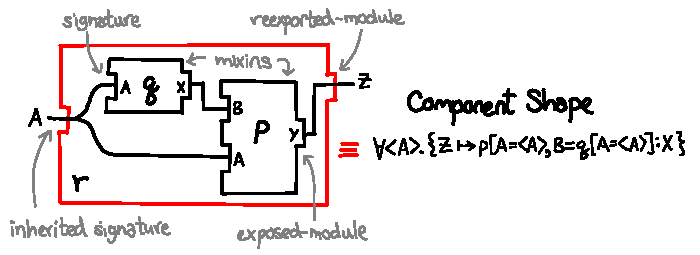
\includegraphics{figures/library-shape-overview.pdf}
\end{figure}

We now formalize mixin linking and describe some of its properties.
In particular, we define two major operations
on component shapes: $\textsf{link}()$, which wires up the components in
two shapes, and $\textsf{rnthin}()$, which thins and renames the input
and output ports of a shape; then, we say how to mixin link a
\ccomp{}.  For an informal description of mixin linking refer
to Section~\ref{sec:overview-mixin}.

\[
\begin{array}{ll}
\DIGresolved{}
&
\begin{array}{l}
\DIGmixed{} \\
\DIGshape{}
\end{array}
\end{array}
\]

% Deferred reporting
% Correct rules for unification

\section{Pictorial interpretation}

We can build upon our graphical language of \uid{}s to specify a graphical
language of \emph{component shapes}, which we used in Section~\ref{sec:overview-mixin}
to informally describe the mixin linking process.  A component shape is simply
a ``bigger box'' which contains some number of \uid{}s:

\begin{figure}[H]
\center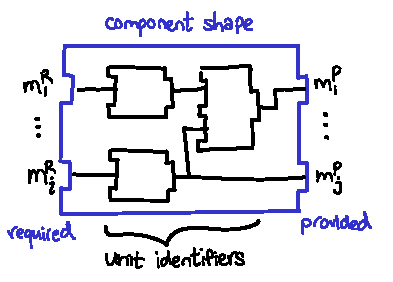
\includegraphics{figures/library-shape-blueprint.pdf}
\end{figure}

\noindent
The required module variables $\reqs = \overline{\hv{m^J_i}}$ can be
read off the diagram by taking the module names of the input ports,
while the provided modules $\provs = \overline{m^P_j \mapsto M_j}$ are a mapping from the module name of each output port to the module identity that is wired to
that port.

These diagrams must obey three rules:

\begin{enumerate}
    \item A wire from a input port cannot go straight to an output port; there
          must be an intervening \uid{}.
    \item No two ports (input or output) can have the same module name.
    \item Every unfilled requirement of a \uid{} must be propagated to the
          requirements of the enclosing component shape.
\end{enumerate}
%
We can restate these rules syntactically:

\begin{definition}[Well-formedness of component shapes] \normalfont{}
A shape $\lctxpair{\provs}{\reqs}$ is \emph{well-formed} if:
\begin{enumerate}
\item It does not provide a module variables
(there is no $m$ such that $\hv{m} \in \textsf{range}(\provs)$),
e.g., $\lctxpair{\{\prov{B}{\hv{A}}\}}{\hv{A}}$ is ill-formed,
\item It does not require what it provides (no $m$
s.t. $\hv{m} \in \reqs$ and $m \in \textsf{dom}(\provs)$),
e.g., $\lctxpair{\{\prov{A}{\MOD{p}{}{A}}\}}{\hv{A}}$ is ill-formed,
\item It is closed; e.g.,
$\lctxpair{\{\prov{B}{\MOD{p}{\subst{A}{\hv{C}}}{B}}\}}{\hv{A}}$ is ill-formed.
\end{enumerate}
\end{definition}

\noindent
Occasionally, we may draw a \uid{} with multiple ports as a shorthand
for two module identifiers which share a \uid{}; although the resulting
box looks similar to a component shape, it is less expressive, since a
component shape can have \emph{different} unit identifiers for the
modules it provides (as can be seen in the above example.)

\section{Linking component shapes}

In our informal description of mixin linking, we simply described mixin
linking as simply ``wiring up'' the input output ports of components;
this wiring operation corresponds to unification in the syntactic realm.

The primary difficulty of specifying mixin linking is handling the
case when multiple component shapes export modules at the same
provided module name.  Although it would be easy to just rule
out this case, we have two goals:

\begin{itemize}
    \item If two distinct modules are brought into the scope with the same
    name, but are never used, this should not be an error.

    \item Mixin linking should be order-invariant, as the source language
    is unordered.
\end{itemize}
%
To handle these problems, we introduce the concept of
\emph{provided module sets} $\Pi ::= \overline{m \mapsto \overline{M}}$,
which is a mapping from module names to sets of module identities
(as opposed to a single module identity, as is the case for a component shape).
We define two operations on provided module sets:

\begin{itemize}
\item Any set of provided modules $\provs$ can be injected into provided module sets $\Pi$ by taking $\Pi(m) = \{ \provs(m) \}$ for all $m \in \dom(\provs)$.

\item Provided module sets can be merged pointwise: $\bigoplus_i \Pi_i = \Pi$ where $\dom(\Pi) = \bigcup_i \dom(\Pi_i) \land\forall m \in \dom(\Pi).\, \Pi(m) = \bigcup_i \Pi'_i(m)$, where $\Pi'_i(m) = \Pi_i(m)$ when $m \in \dom(\Pi_i)$, and $\Pi'_i(m) = \varnothing$ otherwise.
\end{itemize}
%
We now define an $n$-ary linking operation on sets of component shapes: $\textsf{link}(\overline{\lctxpair{\provs_i}{\reqs_i}})$, which produces a substitution and a new component shape as follows:

\begin{enumerate}
    \item Let the provided module sets of all shapes be $\Pi = \bigoplus \provs_i$.
    \item Let the required module variables be $\reqs_\mathsf{all} = \bigcup \reqs_i$.
    \item The requirements which are filled are $\reqs_\mathsf{filled} = \reqs_\mathsf{all} \cap \dom(\Pi)$.
    \item For each $m_i \in \reqs_\mathsf{filled}$, unify $\hv{m_i}$ with each module identity in $\Pi(m_i)$.  (Thus, provided modules which are not used remain ununified.)  Let the overall substitution produced be $S$.
    \item The remaining requirements are $\reqs = \reqs_\mathsf{all} - \reqs_\mathsf{filled}$.  Check that $\substw{\reqs}{S} = \reqs$ (unification did not cause a requirement to be implicitly filled.)
    \item Let $\provs(m) = \Pi(m)$ for all $m$ such that $\Pi(m) = \{ M \}$ for some $M$ (i.e., take the singleton module sets.)
    \item Return new substitution $S$, and new shape $\lctxpair{\provs}{\reqs}$
\end{enumerate}
%
\paragraph{A little design discussion} Unfortunately, this merging operation is not compositional (i.e., cannot be decomposed into a series of binary merge operations); consider the
merge of these shapes: (1) $\lctxpair{ \prov{A}{\MOD{p}{\subst{H}{\hv{H}}}{A}} }{ \hv{H} }$,
(2) \prov{A}{\MOD{p}{\subst{H}{\MOD{q}{}{H}}}{A}}, (3) $\lctxpair{\varnothing}{\hv{A}}$
and (4) \prov{H}{\MOD{q}{}{H}}.
Shapes 1--3 cannot merge together by themselves (we can unify
the \modname{A}s, but as \modname{H} is never
filled we reject the shape in step (5)). Merging these shapes simulateously
with shape 4 solves this problem.

There are a few obvious alternative designs which do not work.
We cannot say that the result of unifying shapes 1--2 is shape 2 (i.e.,
\modname{H} is filled due to the unification of \modname{A}), because
then we would then allow a merge with the shape \prov{H}{\MOD{q}{}{H2}} (call this
shape 4'),
whereas if shape 1 merged with shape 4' first, the identity at \modname{A} would refine
to one that was incompatible with shape 2.

One alternative design that does work and is compositional is to associate a
component shapes with a context which accumulates constraints on module
holes which were not otherwise filled.  When the hole is eventually filled
by a proper requirement, we check that those constraints are satisfied.
But in the end, we probably would like to enforce that all constraints are
discharged when computing a final component shape, at which point the algorithm
ends up being the same as the $n$-ary variant above.

\section{Thinning and renaming component shapes}

%   There is an interesting counterexample showing that linking is not
%   associative:

%   \begin{enumerate}
%   \item $\{ \prov{A}{\cidl{p}[]} \}$
%   \item $\lctxpair{ \prov{B}{\Mod{\cidl{q}[\subst{A}{\hv{A}}]}{B}}, \prov{C}{\Mod{\cidl{q}[\subst{A}{\hv{A}}]}}{C} }{\hv{A}}$
%   \item $\{ \prov{B}{\Mod{\cidl{q}[\subst{A}{\cidl{p}[]}]}{B}} \}$
%   \end{enumerate}

%   Linking (1) and (2), and then (3) works, but linking (2) and (3) does
%   not, as the provisions are required to 

\begin{definition}[Thinning and renaming component shapes] \normalfont{}
We define $\textsf{rnthin}$ on a shape $\lctx$, a total
module renaming $r_R$ and a partial module renaming $r_P$ as follows:
\label{def:rnthin}
  \[
  \begin{array}{l@{\;\;=\;\;}l}
    \Frename{r_R}{\lctxpair{\provs}{\overline{\hv{m_i}}^i}}{r_P}
    % \substw{\substw{r_P^{-1}}{\provs}}{r_R}
    & \lctxpairx%
        {\overlinej{\prov{r_P(m'_j)}{\substw{\provs(m'_j)}{r_R}}}}
        {\overlinei{\holevar{r_R(m_i)}}} \\
    \multicolumn{2}{l}{\quad \textsf{where}~\textsf{dom}(r_P) = \overlinej{m'_j} } \\
  \end{array}
  \]
\end{definition}
%
Intuitively, $r_R$ applies a renaming on all of the input ports of
the component shape, while $r_P$ applies a renaming on the output ports
of a component shape.  $r_R$ must be total because we are not allowed
to ``drop'' any requirements; furthermore when we rename a requirement
we must also rename each reference to it in the provided $M$s.  $r_P$
does not have to be total, and the resulting output ports of the
component shape will only be those mentioned in $r_P$.

For example, if you have a component shaped
$\lctxpairx{\provMOD{A}{p}{\subst{A}{\holevar{B}}}{A},
\provMOD{C}{q}{}{C} }{\modname{B}}$ and you apply the renaming
$(\Sas{A}{X})$ $\texttt{requires}$ $(\Sas{B}{Y})$, we should get a new shape
$\lctxpairx{\provMOD{X}{p}{\subst{A}{\holevar{Y}}}{A}}{\modname{Y}}$.

\begin{figure}[H]
\center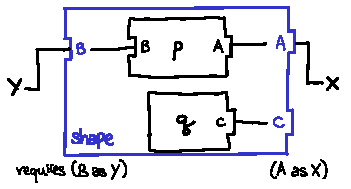
\includegraphics{figures/mixin-renaming-ex.pdf}
\end{figure}

\section{Component mixin linking}

\begin{figure}


\fbox{$\shctx \vdash \Scomp \leadsto \Uunit \haspr \lctx$}

\[
\frac{
\begin{array}{c}
  % \prereqs = \Freqs{\mathtt{component}\: p\: \{ \overline{I_i}^i; \overline{D_j}^j \}} \qquad
  % P = p(\prereqs) \\
  P = p[\reqs] \qquad
  \forall i:\; \shctx; P \vdash \Sdecl_i \leadsto \Uudecl_i \haspr \lctx_i \\
  (S, \lctx) = \Flink{\overlinei{\lctx_i}} \qquad
  \lctxpair{\provs}{\reqs} = \lctx \qquad
  % \provs = \{\overlinej{m_j \mapsto M_j}\}\qquad
  r_P = \overlinei{\Fprovs{\Sdecl_i}} \\
\end{array}
}{
  \shctx \vdash \Scomponent{p}{\overlinei{\Sdecl_i}}
    \leadsto \UsynUnit{p}{\reqs}{\overlinei{\substw{\Uudecl_i}{S}}}
    \haspr \Frename{\,\cdot\,}{\lctx}{r_P}
}
\]
\\


\fbox{$\shctx; P \vdash \Sdecl \leadsto \Uudecl \haspr \lctx$}

%   \[
%   \begin{array}{rcll}
%   &\vdash_\mathsf{ex}& \verb|exposed-module|\: m &\Rightarrow (m, m) \\
%   &\vdash_\mathsf{ex}& \verb|reexported-module|\: m_0\: \mathtt{as}\: m &\Rightarrow (m_0, m) \\
%   \end{array}
%   \]
\[
\frac{
p \haspr \lctx \in \Delta \qquad
\lctx = \lctxpair{\provs}{\reqs} \qquad
(r_R, r_P) = \textsf{getrns}(\lctx, \I{rns}) \qquad
\lctx' = \Frename{r_R}{\lctx}{r_P}
}{
\shctx; P \vdash\Sinclude{p}{\I{rns}} \leadsto \UsynDep{p[r_R]}{r_P} \haspr \lctx'
}
\]
\[
\begin{array}{ll@{\;\;}llll}
  \shctx; P &\vdash&\Sexposed{m}{\Uhsbody} &\leadsto
    & \UsynMod{m}{\Uhsbody} &\;\;\haspr\;\; \{\provMod{m}{P}{m}\} \\
  \shctx; P &\vdash&\Sother{m}{\Uhsbody} &\leadsto
    & \UsynMod{m}{\Uhsbody} &\;\;\haspr\;\; \{\provMod{m}{P}{m}\} \\
  \shctx; P &\vdash&\Srequired{m}{\Uhssig} &\leadsto
    & \UsynSig{m}{\Uhssig} &\;\;\haspr\;\; \lctxpairx{\shnull}{\hv{m}} \\
  \shctx; P &\vdash&\Sreexported{m}{m'} &\leadsto
    & \varnothing &\;\;\haspr\;\; \{\} \\
\end{array}
\]
\caption{Component mixin linking. We implicitly lift $\Theta = \overline{\protect\hv{m}}$
into a substitution $\overline{\protect\subst{m}{\protect\hv{m}}}$.}
\label{fig:mix-in}
\end{figure}

Given $\textsf{link}()$ and $\textsf{rnthin}()$, we are well equipped to say how to mixin link
an entire \ccomp{} (Figure~\ref{fig:mix-in}).  Our general strategy will be to compute the
component shape of every $\I{rdecl}$ (as well as its elaboration to
$\mdecl$) and link them all together in the component judgment,
combining all of the $\mdecl$s together to form the final
elaborated \unit{}.  There is an auxiliary definition (Definition~\ref{def:provs})
which computes the final renaming on the provisions of the
component, so that only \texttt{exposed-module}s and \texttt{reexported-modules}
are exposed to the world.

The rules for shaping modules and signatures are straightforward: a
module $m$ provides the module identity $\Mod{P}{m}$, where $P$ is the
component identity of the component currently being shaped; a signature
$m$ adds a requirement $\hv{m}$.  The rule for includes is more
interesting: we look up the shape of the included unit from the context ($\shctx$),
and then rename it according to the user provided renamings $\I{rns}$.
There is an auxiliary definition (Definition~\ref{def:getrns}) for
translating renaming syntax into a pair of module renamings.

Our presentation of the judgment is slightly
nondeterministic in that it assumes we know the set of requirements
$\Theta$ upfront to compute $P$; however it's easy to see that $P$ is
only used for the module identities assigned to module declarations, and
thus does not actually affect the final requirements of a component.
In practice, $\Theta$ might be computed by a pre-shaping pass.

\begin{definition}[Interpretation of thinning and renaming] \normalfont{}
\label{def:getrns}
\[
  \begin{array}{l@{\;\;=\;\;}l}
    \textsf{getrns}(\lctxpair{\provs}{\reqs}, [\Slparen\overline{\I{rn}_P}\Srparen]~[\texttt{requires}~ \Slparen\overline{\I{rn}_R}\Srparen])
    & (r_P, r_R)
  \end{array}
\]
The syntactic \texttt{include} declaration specifies renamings for
provisions and requirements, but users are allowed to omit a renaming
altogether (in which case everything is brought into scope) or give
only a partial requirement renaming (in which case the requirement
renaming is extended to be total over $\reqs$.)
\textsf{getrns} simply computes the appropriate $r_R$ and $r_P$
given this syntax.
\end{definition}

\begin{definition}[Interpretation of exposed/reexported modules] \normalfont{}
\label{def:provs}
\[
  \begin{array}{l@{\quad=\quad}l}
    \Fprovs{\Sexposed{m}{\_}} & \prov{m}{m} \\
    \Fprovs{\Sreexported{m}{m'}} & \prov{m}{m'} \\
    \Fprovs{\_} & \cdot \\
  \end{array}
\]
Only modules specified with \texttt{exposed-module} or
\texttt{reexported-\allowbreak{}module} should be put in the final shape of
a component.  \textsf{provs} computes the appropriate $r_P$ based
on these declarations.
\end{definition}
